\documentclass{beamer}
\usepackage[utf8]{inputenc}
\usepackage[T1]{fontenc}
\usepackage{algorithm}
\usepackage{algpseudocode}
\usepackage{listings}
\usepackage{xcolor}
\usepackage{tikz-qtree}
\usetikzlibrary{trees}

\definecolor{codegreen}{rgb}{0,0.6,0}
\definecolor{codegray}{rgb}{0.5,0.5,0.5}
\definecolor{codepurple}{rgb}{0.58,0,0.82}
\definecolor{backcolour}{rgb}{0.95,0.95,0.92}

\lstdefinestyle{mystyle}{
   backgroundcolor=\color{backcolour},   
   commentstyle=\color{codegreen},
   keywordstyle=\color{magenta},
   numberstyle=\tiny\color{codegray},
   stringstyle=\color{codepurple},
   basicstyle=\tiny\ttfamily,
   breakatwhitespace=false,         
   breaklines=true,                 
   captionpos=b,                    
   keepspaces=true,                 
   numbers=left,                    
   numbersep=5pt,                  
   showspaces=false,                
   showstringspaces=false,
   showtabs=false,                  
   tabsize=2
}
\lstset{style=mystyle}

\renewcommand{\t}{\text}

\usetheme{Boadilla}
\usecolortheme{seahorse}

\title{Korection deux frases incorecte an frases corecte}
\author{Hurot Eliott - 28537} 
\date{2025}
%\logo{\includegraphics[height=1cm]{}}

\begin{document}

\tikzset{
edge from parent fork down,
level distance=1.75cm,
every tree node/.style={align=center}
}

\frame{\titlepage}

\begin{frame}{Problématique}
   \begin{center}
      \huge{Comment peut-on écrire un programme qui corrige des phrases en français ?}
   \end{center}
\end{frame}

\begin{frame}
   \frametitle{Sommaire}
   \tableofcontents
\end{frame}

\section{Objectif}
\begin{frame}
   \frametitle{Objectif du projet}
   \begin{algorithm}[H]
      \caption{Correction de phrases}
      \begin{algorithmic}
         \Require Phrase à corriger - string
         \Ensure Phrase corrigée - string
      \end{algorithmic}
   \end{algorithm}
\end{frame}

\section{Présentation de l'algorithme}
\begin{frame}
   \frametitle{Etapes :}
   \begin{enumerate}
      \item[\Large{1}] \Large{Analyse lexicale (Lexing)}
      \item[2] \Large{Analyse syntaxique (Parsing)}
      \item[3] \Large{Vérification de la phrase}
      \item[4] \Large{Correction de la phrase}
   \end{enumerate}
\end{frame}

\subsection{Stockage des données}
\begin{frame}
   \frametitle{Stockage des données - Trie}
   Trie ?\\
   Structure de donnée qui prend avantage de la similitude entre les clés
\end{frame}

\begin{frame}
   \frametitle{Exemple}
   \begin{center}
   je - joue - jouer - mire - jouais\\
   \end{center}
   \centering
   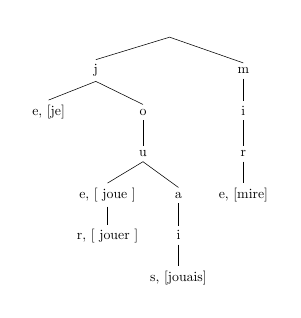
\begin{tikzpicture}[scale=0.5]
   \Tree [.{ }
      [.j 
         [.{e, [je]} ]
         [.o 
            [.u 
               [.{e, [ joue ]}
                  [.{r, [ jouer ]} ] ]
               [.a 
                  [.i 
                     [.{s, [jouais]} ] ] ] ] ] ]
      [.m
         [.i
            [.r
               [.{e, [mire]} ] ] ] ] ]
   \end{tikzpicture}\\
   Taille : 983809 \; \; Hauteur : 39
\end{frame}

\subsection{Analyse lexicale}
\begin{frame}
   \frametitle{Analyse lexicale}
   \begin{algorithm}[H]
      \caption{Analyse lexicale}
      \begin{algorithmic}
         \Require Phrase à corriger - string
         \Ensure Liste de tokens - token list list
      \end{algorithmic}
   \end{algorithm}
   Token : Classe grammaticale, valeur, informations\bigbreak
   Pourquoi token list list ?\\
   Plusieurs sens possibles pour un même mot
\end{frame}

\begin{frame}
   \frametitle{Exemple}
   le petit chat rouge joue\bigbreak
   \begin{tabular}{c c c c c c c}
      [D : le, &, [A : petit, &, [N : chat] &, [A : rouge, &, [V : joue, \\
       ~ Ov : le] & ~ ~ N : petit] & & ~ ~ N : rouge] & ~ ~ V : joue]
   \end{tabular}
   \bigbreak
   Complexité ?\\
   O(n * s)\\
   n : nombre de mots dans la phrase
   s : taille du mot le plus long de la phrase
\end{frame}

\subsection{Analyse syntaxique}
\begin{frame}
   \frametitle{Analyse syntaxique}
   \begin{algorithm}[H]
      \caption{Analyse syntaxique}
      \begin{algorithmic}
         \Require Liste de tokens - token list list
         \Ensure Arbre syntaxique - syntax\_tree list
      \end{algorithmic}
   \end{algorithm}
\end{frame}

\begin{frame}[fragile]
    \frametitle{Définition des structures}

    \begin{lstlisting}[
        language=C
    ]
struct cell
{
    float T; // --------------- en degre Celsius
    char* type; // ------------ type de la cellule (airExt, airInt, wall, window, door)
    coord co; // -------------- coordonnees de la cellule
    float CTherVol; // -------- Capacite thermique volumique en J.K-1.m-3
    float lambda; // ---------- Conductivite thermique en W.K-1.m-1
    float surface; // --------- Surface en m2
    float epaisseur; // ------- Epaisseur en m
    float lambda_iso_ext; // -- Conductivite thermique de l'isolant exterieur en W.K-1.m-1
    float lambda_iso_int; // -- Conductivite thermique de l'isolant interieur en W.K-1.m-1
    float epaisseur_iso_ext; // Epaisseur de l'isolant exterieur en m
    float epaisseur_iso_int; // Epaisseur de l'isolant interieur en m
};
    \end{lstlisting}

\end{frame}

\end{document}
